\documentclass{tufte-handout}

\usepackage{/Users/paulallen/OU/Astronomy/style}
\usepackage{tensor}
\usepackage{leftidx}
% Define a new command for subscripts and superscripts
\newcommand{\subsup}[3]{{#1}_{\tensor*[^{#2}]{#3}{}}}
\usepackage[table]{xcolor}% http://ctan.org/pkg/xcolor
\usetikzlibrary{matrix} % <-- needed for matrix of nodes
\usetikzlibrary{calc}   % <-- optional, can sometimes be helpful



\begin{document}
\tma{05}

\begin{question}

\qpart

    A Segre chart to show the nuclear reactions on the s-process pathway from \( \leftidx{^{121}}{Sb} \rightarrow \leftidx{^{121}}{Xe} \)

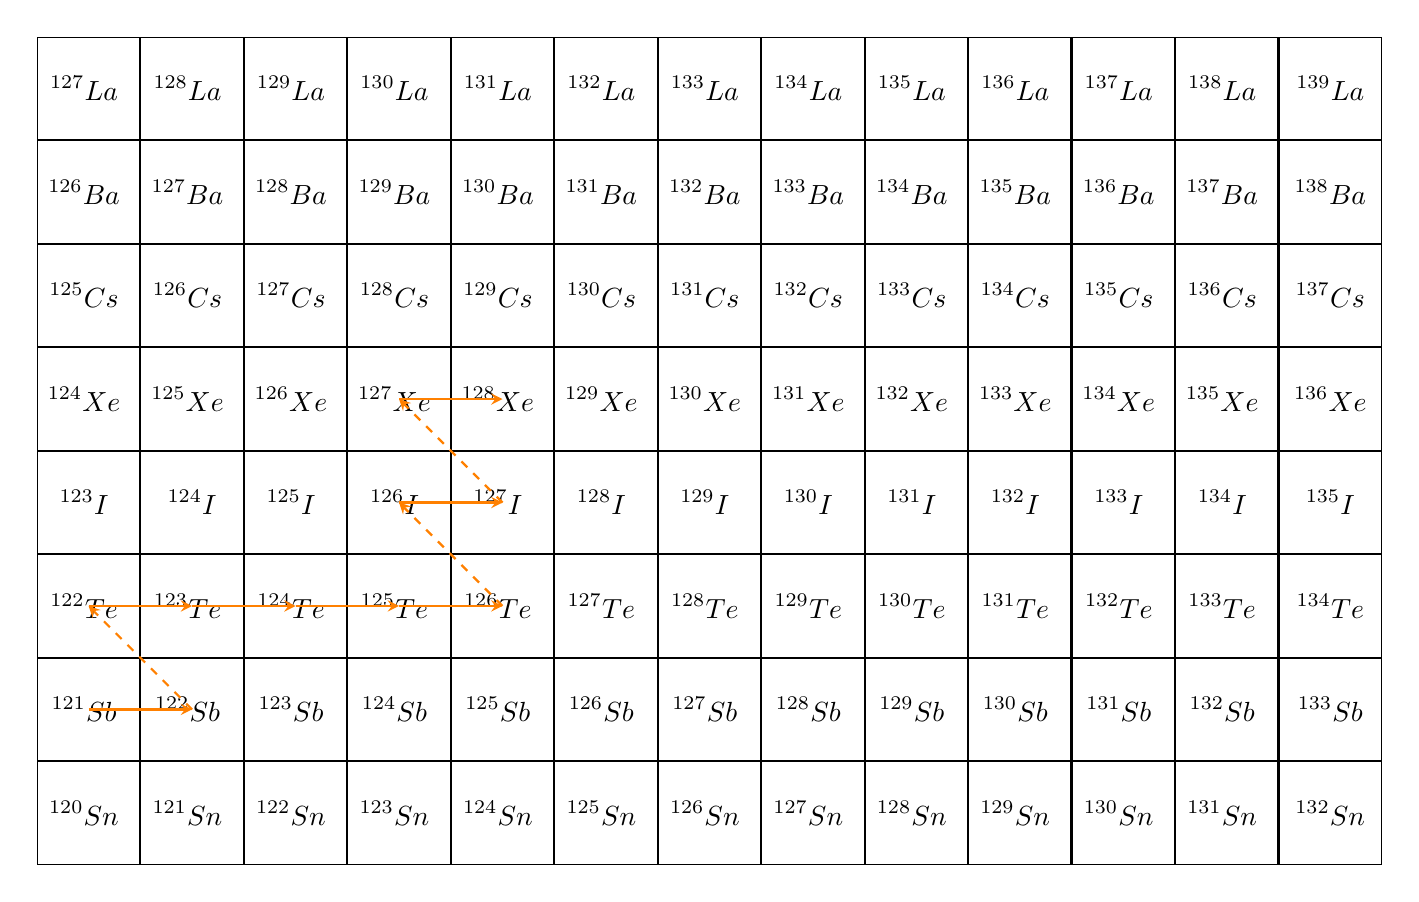
\begin{tikzpicture}[>=stealth]

    
% 1. Define a style for your "boxed" nodes
    \tikzset{
isotope/.style={
    draw,              % draw a border
    rectangle,         % rectangular shape
    minimum width=1.3cm, % tweak as needed
    minimum height=1.3cm,
    align=center       % center the text inside
}} 

% 2. Define the isotope nodes
\matrix (m) [
    matrix of nodes,
    nodes={isotope}
]{
    \( \leftidx{^{127}}{La} \) & \( \leftidx{^{128}}{La} \) &  \( \leftidx{^{129}}{La} \) & \( \leftidx{^{130}}{La} \) & \( \leftidx{^{131}}{La} \) &
        \( \leftidx{^{132}}{La} \) & \( \leftidx{^{133}}{La} \) & \( \leftidx{^{134}}{La} \) &\( \leftidx{^{135}}{La} \) & \( \leftidx{^{136}}{La} \) &
        \( \leftidx{^{137}}{La} \) & \( \leftidx{^{138}}{La} \) & \( \leftidx{^{139}}{La} \)\\
    \( \leftidx{^{126}}{Ba} \) & \( \leftidx{^{127}}{Ba}\) & \( \leftidx{^{128}}{Ba} \) & \( \leftidx{^{129}}{Ba} \) & \( \leftidx{^{130}}{Ba} \) &
        \( \leftidx{^{131}}{Ba} \) & \( \leftidx{^{132}}{Ba} \) & \( \leftidx{^{133}}{Ba} \) & \( \leftidx{^{134}}{Ba} \) & \( \leftidx{^{135}}{Ba} \) &
        \( \leftidx{^{136}}{Ba} \) & \( \leftidx{^{137}}{Ba} \) & \( \leftidx{^{138}}{Ba} \)\\
    \( \leftidx{^{125}}{Cs}\) & \(\leftidx{^{126}}{Cs}\) & \(\leftidx{^{127}}{Cs}\) &\( \leftidx{^{128}}{Cs}\) & \(\leftidx{^{129}}{Cs}\) &
        \( \leftidx{^{130}}{Cs} \) & \( \leftidx{^{131}}{Cs} \) & \( \leftidx{^{132}}{Cs} \) & \( \leftidx{^{133}}{Cs} \) & \( \leftidx{^{134}}{Cs }\) &
        \( \leftidx{^{135}}{Cs} \) & \( \leftidx{^{136}}{Cs} \) & \(\leftidx{^{137}}{Cs} \)\\
    \( \leftidx{^{124}}{Xe} \) & \( \leftidx{^{125}}{Xe} \) & \( \leftidx{^{126}}{Xe} \) & \( \leftidx{^{127}}{Xe} \) & \( \leftidx{^{128}}{Xe} \) &
        \( \leftidx{^{129}}{Xe} \) & \( \leftidx{^{130}}{Xe} \) & \( \leftidx{^{131}}{Xe} \) & \(\leftidx{^{132}}{Xe} \) & \( \leftidx{^{133}}{Xe} \) &
        \( \leftidx{^{134}}{Xe} \) & \( \leftidx{^{135}}{Xe} \) & \( \leftidx{^{136}}{Xe} \)\\
    \( \leftidx{^{123}}{I}\) & \(\leftidx{^{124}}{I} \)& \(\leftidx{^{125}}{I}\) &\( \leftidx{^{126}}{I}\) &\( \leftidx{^{127}}{I}\) &
        \( \leftidx{^{128}}{I} \) & \( \leftidx{^{129}}{I} \) & \( \leftidx{^{130}}{I}\) & \( \leftidx{^{131}}{I} \) & \(\leftidx{^{132}}{I} \) &
        \( \leftidx{^{133}}{I} \) & \( \leftidx{^{134}}{I} \) & \( \leftidx{^{135}}{I} \)\\
    \( \leftidx{^{122}}{Te} \) & \( \leftidx{^{123}}{Te} \) & \( \leftidx{^{124}}{Te} \) & \( \leftidx{^{125}}{Te} \) & \( \leftidx{^{126}}{Te} \) &
        \( \leftidx{^{127}}{Te} \) & \( \leftidx{^{128}}{Te} \) & \( \leftidx{^{129}}{Te} \) & \( \leftidx{^{130}}{Te}\) &\( \leftidx{^{131}}{Te}\) &
        \( \leftidx{^{132}}{Te} \) & \( \leftidx{^{133}}{Te} \) & \( \leftidx{^{134}}{Te} \)\\
    \( \leftidx{^{121}}{Sb} \) & \( \leftidx{^{122}}{Sb} \) & \( \leftidx{^{123}}{Sb} \) & \( \leftidx{^{124}}{Sb} \) & \( \leftidx{^{125}}{Sb} \) &
        \( \leftidx{^{126}}{Sb} \) & \( \leftidx{^{127}}{Sb} \) & \( \leftidx{^{128}}{Sb} \) & \( \leftidx{^{129}}{Sb} \) & \( \leftidx{^{130}}{Sb} \) &
        \( \leftidx{^{131}}{Sb} \) & \( \leftidx{^{132}}{Sb} \) & \( \leftidx{^{133}}{Sb} \)\\
    \( \leftidx{^{120}}{Sn} \) & \( \leftidx{^{121}}{Sn} \) & \( \leftidx{^{122}}{Sn} \) & \( \leftidx{^{123}}{Sn} \) & \( \leftidx{^{124}}{Sn} \) &
        \( \leftidx{^{125}}{Sn} \) & \( \leftidx{^{126}}{Sn} \) & \( \leftidx{^{127}}{Sn} \) & \( \leftidx{^{128}}{Sn} \) & \( \leftidx{^{129}}{Sn} \) &
        \( \leftidx{^{130}}{Sn} \) & \( \leftidx{^{131}}{Sn} \) & \( \leftidx{^{132}}{Sn} \)\\
        };
 
% 3. Connect the nodes in the matrix with arrows.
        \draw[->, thick, orange] (m-7-1.center) -- (m-7-2.center);
        \draw[->, dashed, thick, orange] (m-7-2.center) -- (m-6-1.center);
        \draw[->, thick, orange] (m-6-1.center) -- (m-6-2.center);
        \draw[->, thick, orange] (m-6-2.center) -- (m-6-3.center);
        \draw[->, thick, orange] (m-6-3.center) -- (m-6-4.center);
        \draw[->, thick, orange] (m-6-4.center) -- (m-6-5.center);
        \draw[->, dashed, thick, orange] (m-6-5.center) -- (m-5-4.center);
        \draw[->, thick, orange] (m-5-4.center) -- (m-5-5.center);
        \draw[->, dashed, thick, orange] (m-5-5.center) -- (m-4-4.center);
        \draw[->, thick, orange] (m-4-4.center) -- (m-4-5.center);
\end{tikzpicture}

\vspace{2cm}

\begin{itemize}
    \item \( \leftidx{^{121}}{Sb} \rightarrow \leftidx{^{122}}{Sb} \) is a neutron capture.\\
    \item \( \leftidx{^{122}}{Sb} \rightarrow \leftidx{^{122}}{Te} \) undergos beta minus decay.\\
    \item \( \leftidx{^{122}}{Te} \rightarrow \leftidx{^{123}}{Te} \rightarrow \leftidx{^{124}}{Te} \rightarrow \leftidx{^{125}}{Te} 
    \rightarrow \leftidx{^{126}}{Te}\) each of these steps is a neutron capture.\\
    \item \( \leftidx{^{126}}{Te} \rightarrow \leftidx{^{126}}{I} \) is a beta minus decay.\\
    \item \( \leftidx{^{126}}{I} \rightarrow \leftidx{^{127}}{I} \) is another neutron capture.\\
    \item \( \leftidx{^{127}}{I} \rightarrow \leftidx{^{127}}{Xe} \) is a beta minus decay.\\
    \item and finally \( \leftidx{^{127}}{Xe} \rightarrow \leftidx{^{128}}{Xe} \) is a neutron capture.\\
\end{itemize}

\clearpage

\qpart

\qsubpart
Luminous blue variable stars are massive, evolved stars that show dramatic variations in luminosity. 
They are thought to be in a transitional phase between the main sequence and Wolf-Rayet stars. 
They are characterised by their high luminosity, mass loss and spectral variability. 
They are thought to be the progenitors of supernovae and gamma-ray bursts.

\vspace{2cm}

\qsubpart

As massive stars evolve off the main sequence and start burning heavier elements in their cores, they expand significantly, 
becoming cooler and thus shifting horizontally to the right, toward the red supergiant region of the HR diagram.

\vspace{2cm}

\qsubpart

High mass stars are more luminous and have a higher temperature than low mass stars, this can cause strong stallar
winds to form, which can cause the star to lose mass. This mass loss can cause the star to become unstable and
eventually explode as a supernova.
HIgh mass stars also have more fuel to burn, and can burn heavier elements in their core, which causes the star to
have shorter life spans than low mass stars.
Higher mass stars can also have transient events which cause them to llose lots of mass very quickly,
but the cause for these is not well known. 

Lower mass stars tend to loose their mass more slowely, mainly through planatary nebulae, and do not have the
mass to burn heavier elements in their core. This means that they have longer life spans than high mass stars.
\end{question}

\clearpage

\begin{question}

\qpart%Graphs
\qpart

\includegraphics[scale=0.75]{graph.png}

From the above graph with the redshift \( 0.05 < z < 0.1 \) we obtain the following equation
\[ \log_{10}\rb{L_{radio}} = 0.5004\rb{\log_{10}\rb{SFR}} + 30.475 \]

\clearpage

\qpart

\begin{align*}
\stext{Hence for a galaxy with a SFR of \( \SI{20}{\Ms\year} \) within this redshift range}
    \log_{10}\rb{L_{radio}} &= 0.5004\rb{\log_{10}\rb{SFR}} + 30.475 \\
\stext{Substuting in our values}
    \log_{10}\rb{L_{radio}} &= 0.5004\rb{\log_{10}\rb{20}} + 30.475 \\
    L_{radio} = 10^{0.5004\rb{\log_{10}\rb{20}} + 30.475} &= 10^{0.5004\rb{1.3010} + 30.475} \\
    &= 10^{0.6510 + 30.475} \\
    &= 10^{31.1260} \\
    &= \SI{1.34e31}{\W}
\snote{To 3 s.f}
\end{align*}

Considering from the unsorted data we ued the following equation;

\begin{align*}
    \log_{10}\rb{L_{radio}} &= 0.9628\rb{\log_{10}\rb{SFR}} + 30.368 \\
\stext{Substuting in our values}
    \log_{10}\rb{L_{radio}} &= 0.9628\rb{\log_{10}\rb{20}} + 30.368 \\
    L_{radio} = 10^{0.9628\rb{\log_{10}\rb{20}} + 30.368} &= 10^{0.9628\rb{1.3010} + 30.368} \\
    &= 10^{1.2526 + 30.368} \\
    &= 10^{31.6206} \\
    &= \SI{4.17e31}{\W}
\snote{To 3 s.f}
\end{align*}

Hence the two values differ by a factor of \( \frac{4.17}{1.34} = 3.12 \), which is a significant difference.
Therefore it is nescesaary to consider the redshift range when calculating the radio luminosity of a galaxy.
Because this will remove outliers in the data possibly causing stochastic effects from the small number of galaxies in the sample.

\clearpage

\qpart

Using 

\[ R_{SN} = 0.007 \times SFR \]

And looking at a star forming galaxy with a supernova rate of 3 per century, we can calculate the SFR as follows;

\begin{align*}
    R_{SN} &= 0.007 \times SFR \\[8pt]  
    SFR &= \frac{R_{SN}}{0.007} \\[8pt]
    &= \frac{0.03}{0.007} \\[8pt]
    &= \SI{4.29}{\Ms\year}\\[8pt]
\snote{to 3 s.f}\\
\stext{Hence we can find the \( L_{radio} \)}\\[8pt]
    \log_{10}\rb{L_{radio}} &= 0.5004\rb{\log_{10}\rb{4.29}} + 30.475 \\[8pt]
    L_{radio} = 10^{0.5004\rb{\log_{10}\rb{4.29}} + 30.475} \\[8pt]
    &= 10^{0.5004\rb{0.6320} + 30.475} \\[8pt]
    &= 10^{0.3163 + 30.475} \\[8pt]
    &= 10^{30.7913} \\[8pt]
    &= \SI{6.18e30}{\W}\\
\snote{to 3 s.f}
\end{align*}

\end{question}

\end{document}